\subsection{The Web Application}
We will be utilizing AWS' Amplify Console to host our web application which will allow users to view
the data and air quality information collected from the network of sensor nodes. We will be
designing this web application using the JavaScript framework, ReactJS, along with Typescript. Users
will be able to view one or many sensor data map overlays, and can toggle specific overlays, such as
\sdo or \ndo to hide or view them simultaneously. An account won't be required to view sensor data,
but an account will be required to setup a personal node. Users that are owners of sensor nodes will
be able to manage their devices, get detailed status information, and control them remotely through
a graphical (web) user interface or text console. A prototype of how the website might generally
look is shown in figure \ref{fig:website-prototype-map}. 

\begin{figure}
  \centering
  \caption{Web Application Map View Prototype}
  \label{fig:website-prototype-map} 

  \begin{subfigure}[b]{\textwidth}
    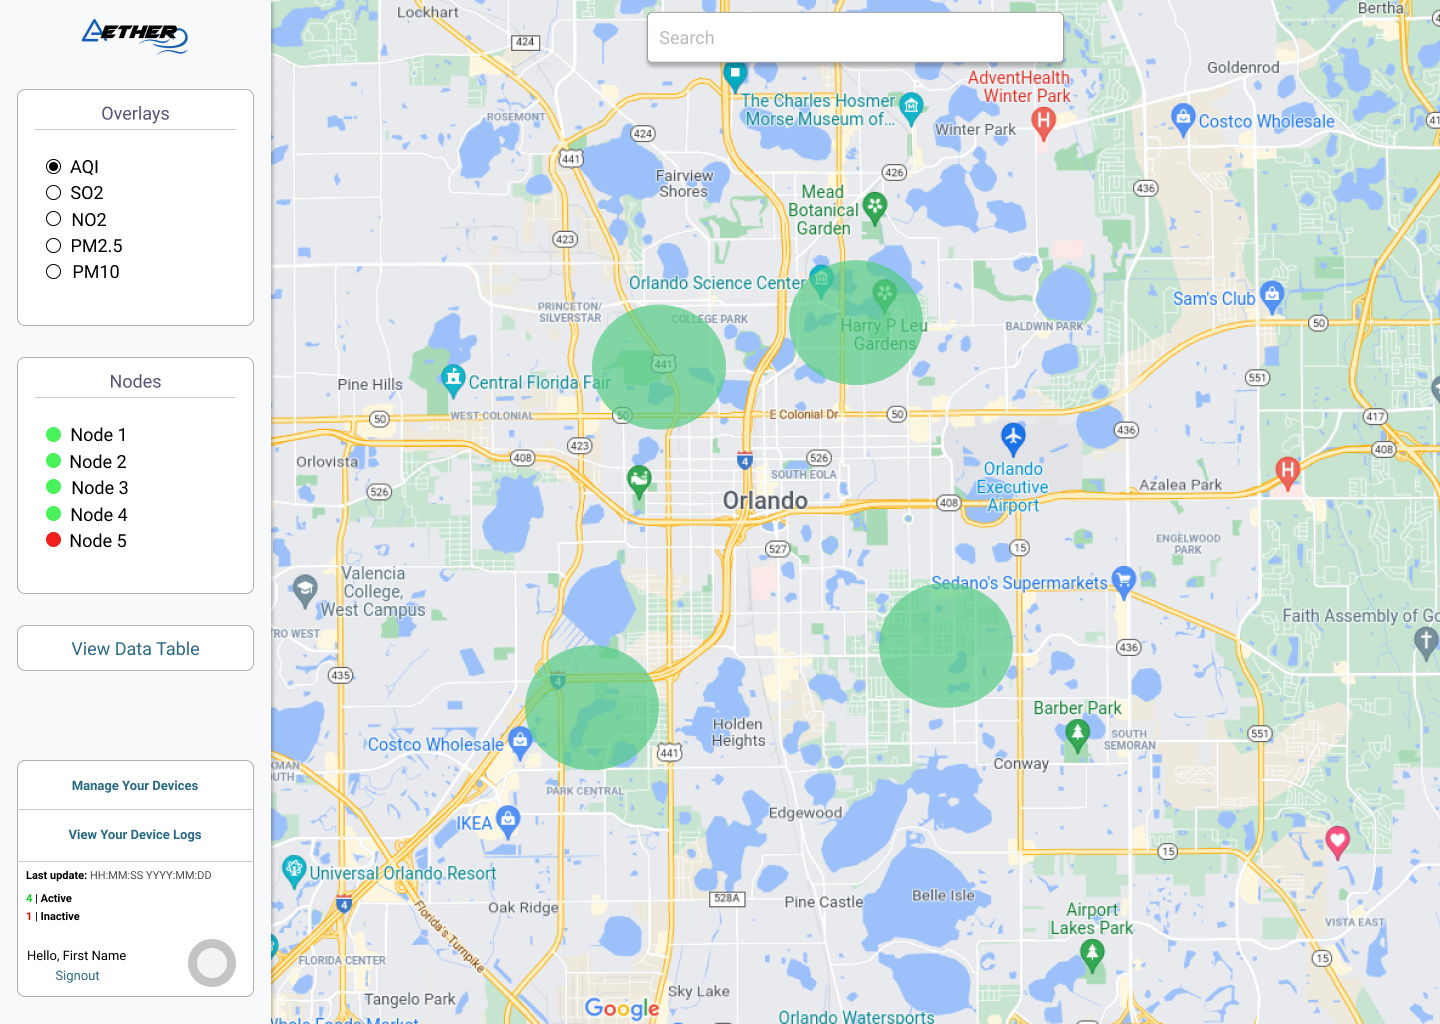
\includegraphics[width=5.5in]{webapp-prototype}
    \caption{Light Mode}
    \label{fig:website-prototype-map-light} 
  \end{subfigure}

  \hfill

  \begin{subfigure}[b]{\textwidth}
    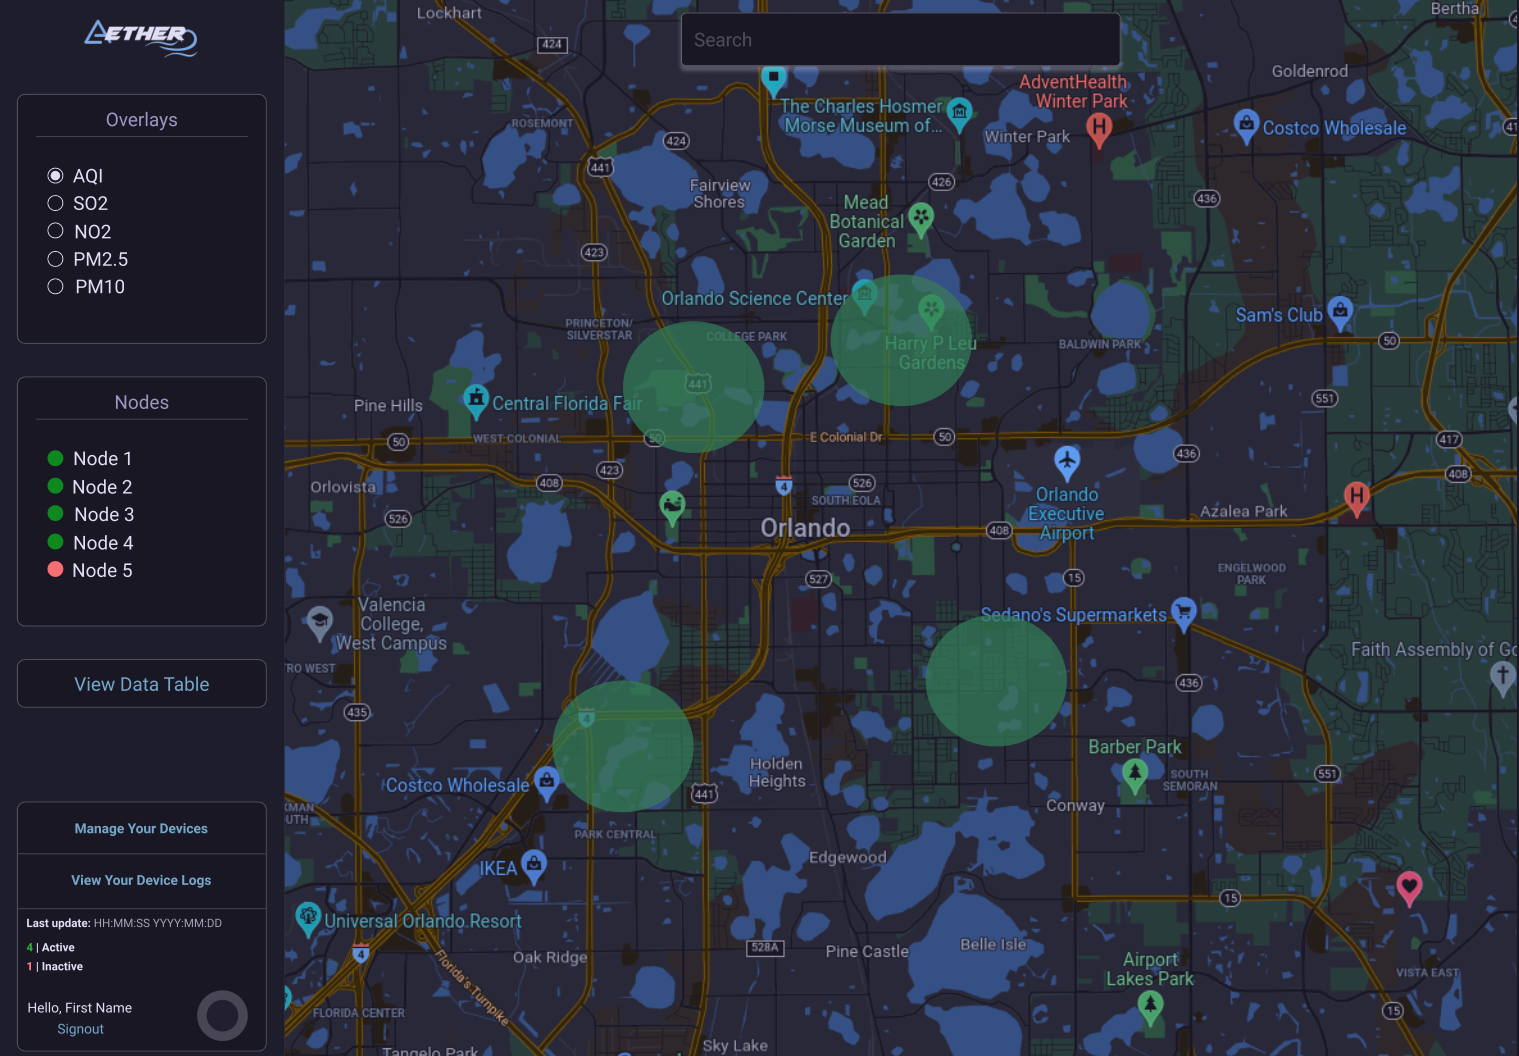
\includegraphics[width=5.5in]{webapp-prototype-dark}
    \caption{Dark Mode}
    \label{fig:website-prototype-map-dark} 
  \end{subfigure}
\end{figure}

The webapp will use an assortment of JavaScript and React libraries to speed up development. The map
service will be provided by Google's Maps API
\footnote{https://developers.google.com/maps/documentation/javascript/overview}. The Google Maps API
allows developers to draw shapes, change the styling of the map, adding custom markers, adding
custom info windows, doing searches, and much more. Google also provides a simple React Google Maps
wrapper component \footnote{https://www.npmjs.com/package/@googlemaps/react-wrapper}.

As for the main UI design, the React Material UI (MUI) library \footnote{https://mui.com} will be
used. MUI provides pre-made UI React components that can be extensively customized. It also supports
advanced theming to create custom color palettes, UI transitions, and the ability to dynamically
change the color scheme of the UI (light or dark mode). MUI also provides a webapp to customize and
generate a color palette that adheres to color theory.

\begin{figure}
  \centering
  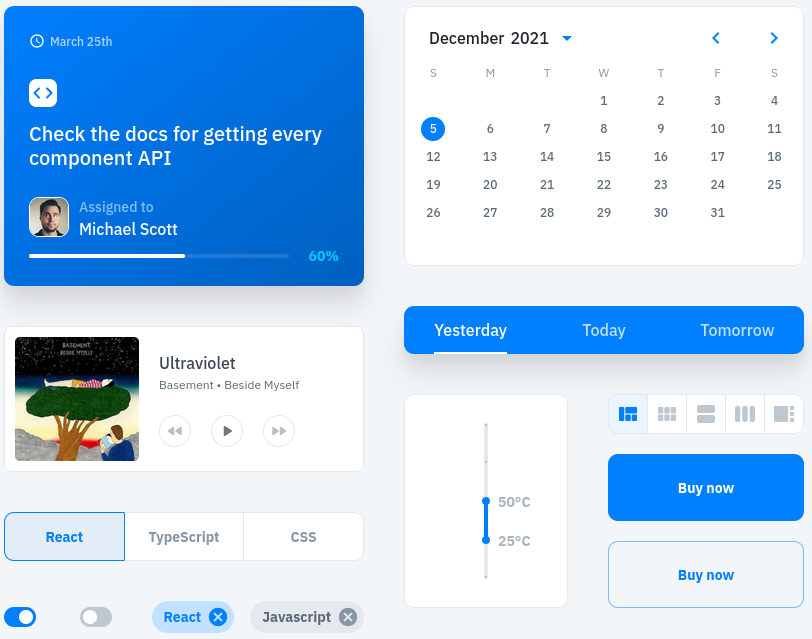
\includegraphics[width=4in]{mui-examples}
  \caption{MUI Component Examples \footnote{Taken from their homepage}}
  \label{fig:mui-example-components} 
\end{figure}

\subsubsection{React}
React is a component-based JavaScript framework for design web application user interfaces. React
components encapsulate the state of a particulate UI component, such as a search box, list, or
toolbar, to make state management and interactivity easier and more responsive. Components in React
are used together in a hierarchical structure, and data is only passed down the hierarchical tree.
Components can be instantiated multiple times allowing for more code re-usability and code
sharability. There is a enormous collection of open source React components available online on
GitHub and NPM (NodeJS Package Manager). Since most React apps are single page applications, meaning
there is only one main server call to get the static assets (i.e. photos, HTML, CSS, JS), and the
rest of the user interface control flow is handled by the client. This is called client routing.
React Router is a library for easily creating dynamic routes for a React app. Different routes are
displayed in the URL (the page isn't reloaded), and dictate which components are shown. For
instance, if a user visits our site,

\code{https://aether.io}

And, had clicked on a sensor node on the map, it would display an info window
overlaid on the map displaying various information about the node. That route might look something
like this:

\code{https://aether.io/node/103653}

Where \code{103653} could be the identifier for that particular node. For example, the subdomain,
\code{node}, could have routes for adding a new node, managing a node, or delete a node.

Lastly, for any time we would need to display charts for sensor data, we will be using a library
called Recharts since it was made for React, and is currently known as the most reliable and is
widely used.


\subsubsection{User Authorization}
User authorization will be carried out with AWS Cognito, which handles user authorization, user
creation, session management, and social logins, such as Facebook or Apple. However, it will be
a stretch goal to have social login. The login and signup UI is handled by Amazon and is served by
their servers, but can be customized to match our theming and styling.

\subsubsection{User Interaction}
The homepage will be a landing page that will have a buttons to go view the map, login, signup, and
information about the project, including documentation and the development team. Users won't need to
signup to use the map, but it will be required if they want to register their device. The map page,
as shown in the prototype in \ref{website-prototype-map}, will ask the user if they want to provide
their geolocation, or they can otherwise search for their location to view sensor data. The exact
locations of the devices won't be displayed unless the user is the owner. On the device management
page, users will be able to see a table of their devices that shows the status of each device, along
with any statistics. Users can click on the row in the table that corresponds to a particular
device to view its logs, geolocation, and send commands to it. From the map page, there will be
a button, shown as "View Data Table" in figures \ref{website-prototype-map}, that will show another
page that shows historical data in tables and graphs for each device and/or zip code.
